\documentclass{article}

\RequirePackage{hyperref}

\usepackage[parfill]{parskip}
\usepackage[letterpaper, portrait, margin=1in]{geometry}
% Author
\usepackage{authblk}
% Images
\usepackage{graphicx}
\usepackage{lscape}
\usepackage{longtable}
% \usepackage{svg}

%\articlesubtype{This is the article type (optional)}
% \bibliography{paper-webserver.bib}

\usepackage{xcolor}
\newcommand\mwcomment[1]{\textcolor{red}{#1}}

\begin{document}


\mwcomment{I would suggest we avoid the comparison to sequence databases or genome sequence platforms (e.g. assembly, gene annotation etc). We really don't have the capacity to replace EnteroBase, Genbank, IRIDA, etc. I see Spfy as a repository of E.coli phenotypes important for public health. It allows users to rapidly predict phenotypes and retrieve the phenotypes of historical strains to: track trends, observe context amoung evolutionary related strains, identify biomarkers, etc. In other words, Spfy provides WGS-based phenotypes + big picture comparative genomics. The big picture is only possible by 1. recomputing everything everytime, or 2. storing the results as genomes are analysed. With size of WGS data, option 2 is only viable option}
\mwcomment{Title may need work. Should it mention comparative genomics? Can't be too long thou}
\title{Spfy: an integrated graph database for real-time prediction of Escherichia coli phenotypes and downstream comparative analyses}

\author[1]{Kevin K Le\thanks{kevin.le@canada.ca}}
\author[1]{Matthew D Whiteside}
\author[1]{James Hopkins}
\author[1]{Victor PJ Gannon}
\author[1]{Chad R Laing\thanks{chad.laing@canada.ca}}
\affil[1]{National Microbiology Laboratory at Lethbridge, Public Health Agency of Canada, Twp Rd 9-1, Lethbridge, AB, T1J 3Z4, Canada}

\renewcommand\Authands{ and }

\maketitle

\begin{abstract}

Public health laboratories are currently moving to whole-genome sequencing based analyses, and require rapid prediction of relevent pathogen phenotypes impacting health. Current workflows in comparative computational genomics rely on chaining different analysis software together, but lack storage and retrieval methods for the generated results.
\mwcomment{Reference laboratories do not care about data retrieval, only real-time results. Researchers care more about context and thus would use a historical record of phenotypes for all predicted strains} 
To solve this problem, we have created Spfy, which uses a graph database to store and retrieve results from computational workflows. The newly developed Spfy platform facilitates rapid phenotype identification, as well as the efficient storage and downstream comparative anlaysis of tens of thousands of genome sequences. Though generally applicable to bacterial genome sequences, Spfy currently contains X \textit{Escherichia coli} genomes, for which \textit{in-silico} serotype and Shiga-toxin subtype, as well as the presence of known virulence factors and antimicrobial resistance determinants have been computed.
Spfy links the results and metadata to the genome sequences through a standardized ontology, which facilitates hypothesis testing in fields ranging from population genomics to epidemiology, while mitigating the recomputing of analyses.
The graph approach is flexible, and can accommodate new analysis software modules as they are developed, and easily link new results to those already stored.
Integrated data storage and analyses are currently necessary as the number of publicly available whole genome sequences is currently in the hundreds of thousands, with millions likely to be available within the next few years. 
\mwcomment{should we mention how many ecoli genomes are available? It might prompt reviewers to ask why we don't have them in spfy}
\par

Database URL: \url{https://lfz.corefacility.ca/superphy/spfy/}.

\end{abstract}


\section{Introduction}
% new outline
% para
% 1. brief: WGS is standard
% 2. Big Problem: but tools are for individual analysis
% 3. 100,000 genomes, (lookup number for Enterobase, GenBank), how do we run analysis on it
% 4. previous methods (Galaxy/IRIDA: real-time, but no storage of results, other website examples - Denmark?), what problems they addressed
% 5. Problems that remain / lack of result storage means: recomputation, lost data, can't reference old analyses, not suited for "big data"
% 6. Solutions in general: store and increment, huga "big data" analyses, parallelization /queues
% para
% 1. Our specific problem, previous work
% 2. Why solving it is important (for Public health / research)
% 3. how we solved it
% para
% 4. benefits: rapid analyses in real-time -> huge comparisons, replace reference labs -> time & money saved, future work -> expand analyses, more genomes, more species
% 5. analyses modules -> conda -> IRIDA/Galaxy
% 6. short snippit on website link & github link

% 1. brief: WGS is standard
Whole genome sequencing (WGS) can in theory provide the entire genetic content of an organism. This unparalleled resolution and sensitivity has recently transformed public-health surveillance and outbreak response \cite{ronholm2016navigating,lytsy2017time}. Additionally, the identification of novel disease mechanisms \cite{wang2014whole,yuen2015whole}, and rapid clinical diagnoses and reference lab tests based on the specific mechanism of disease are now possible. \cite{willig2015whole,dewey2014clinical}.

% 2. Big Problem: but tools are for individual analysis
The rapid characterization and comparison of bacterial pathogens relies principally on the combination of outputs from multiple software programs that are targeted for specific applications. Examples include the identification of known antimircrobial resistance (AMR) genes, through software such as the Resistance Gene Identifier (RGI) \cite{mcarthur2013comprehensive}, \cite{kleinheinz2014applying}, \cite{gupta2014arg}, and ARIBA \cite{hunt2017ariba}; or the identification of known virulence factor genes (VF) through software such as VirulenceFinder \cite{kleinheinz2014applying}, SRST2 \cite{inouye2014srst2}, and GeneSippr \cite{lambert2015genesippr}. For clinical diagnoses and comparisons, individual species can be first divided into subtypes with complementing AMR and VF results. Software methods for subtyping rely on intraspecies genes or genomic regions, and are targeted through software such as Phylotyper \cite{whiteside2017phylotyper}, SerotypeFinder \cite{joensen2015rapid}, the EcOH dataset applied through SRST2 \cite{ingle2016silico}, and V-Typer \cite{carrillo2016comparative}. These methods represent \textit{in-silico} analogues of traditional wet-lab tests, which allows new WGS results to be viewed in the context of historical tests, and greatly expedites the analyses of newly sequenced genomes. 

Comprehensive platforms that combine individual programs into a cohesive whole also exist. These include free platforms such as the Bacterium Analysis Pipeline (BAP) \cite{thomsen2016bacterial}, and the Pathosystems Resource Integration Center (PATRIC) \cite{wattam2016improvements}. Commercial applications, such as Bionumerics, which is used by PulseNet International for the analyses of WGS data in outbreak situations also exist, and offer support as well as accredited, standardized tests \cite{swaminathan2001pulsenet}. These platforms are designed to be applied to individual projects \cite{}.

% 3. 100,000 genomes, (lookup number for Enterobase, GenBank), how do we run analysis on it
WGS of bacterial pathogens have recently accumulated in public databases in the hundreds of thousands, with millions set to be available within the next few years. For \textit{Escherichia coli} alone, there are over sixty thousand publicly available genomes in EnteroBase \url{https://enterobase.warwick.ac.uk/} and three million sequenced genomes in GenBank \cite{doi:10.1093/nar/gks1195}. Many of the comparative analyses that are currently used in the analyses of bacterial genomes are broadly useful, and therefore computed multiple times for the same genomes. An effective method to mitigate the recomputing of analyses, is to make the storage and retrieval of results part of the analyses platform, and effectively linked to the genomes of interest through a standardized ontology. Such measures can help ensure the rapid response times required for public health applications, and allow results to be integrated and progressively updated as new data becomes available.
\mwcomment{should we mention how many ecoli genomes are available? It might prompt reviewers to ask why we don't have them in spfy}

% 4. Our specific problem, previous work
We have previously developed Superphy \cite{whiteside2016superphy}, an online predictive genomics platform targeting \textit{E. coli}. Superphy integrates pre-computed results with domain-specific knowledge to provide real-time exploration of publicly available genomes. While this tool has been useful for the thousands of pre-computed genomes in its database, the current pace of genome sequencing requires real-time predictive genomic analyses of tens-, and soon hundreds-of-thousands of genomes, and the long term storage and referencing of these results, something that the original SuperPhy platform was incapable of.

% ?. Why solving it is important (for Public health / research)
% Merging points from here into the above sections (2,3,4) to avoid repetition
% - everything is being sequenced (surveillance / outbreak / research)
% - previously mentioned common analyses / want to leverage pre-computed results
% - WGS does not discard old methods, linkage to thousands of historical results by developing in-silico methods of traditional tests
% - need fast / standardized outbreak response
% - need fast / standardized in-silico reference lab
% - need fast / standardized storage and retrieval of results based on ontology
% - all known data can be leveraged, allows the most informed decisions possible
% - etc.

% 5. how we solved it
In this study, we present the Spfy update to the SuperPhy platform, which integrates a graph database with real-time analyses; this integration avoids recomputing identical analyses. Graph-based result storage also allows retrospective comparisons as more genomes are sequenced or populations change, and is flexible, accommodating new analysis modules as they are developed. The database is available at \url{https://lfz.corefacility.ca/superphy/spfy/}.

% {needs to be beefed up, in language a biologist / public health worker would care about}

% end of new intro

% **************************************************************
% Keep this command to avoid text of first page running into the
% first page footnotes
\enlargethispage{-65.1pt}
% **************************************************************

% Some general comments
% The NAR Database issue is more of a showcase then a rigorous exploration of software design choices.
% Given this focus, i would suggest the following:
% 1. Increase/highlight the discriptions of the functions and capabilities, maybe by adding a Functionality section
% 2. In the Implmentation (or Methods) section, only give a cursory description of the layout and components. Don't need to provide too much justification
% 3. Use the Results section to highlight the scope/size and speed. This can be short
% 4. In the Discussion, this is where i would expand on the justications and reasons for specific design choices. Pick 2-3 main ones and discuss those (i.e. don't need to justify our choice of documentation software). Also compare with other software in Discussion.
% 5. Add a conclusions section


\section{FUNCTIONALITY}
% ONLY FOCUS ON THE ANALYSIS MODULES
% Describe available functions in spfy
% para covering everything

Spfy provides rapid in-silco versions of common reference laboratory tests for the analyses of \textit{E. coli}. It supports the following \textit{in-silico} subtyping options: serotyping, through both O- and H-antigen identification {ectyper ref}; Shiga-toxin 1 (Stx1), Shiga-toxin 2 (Stx2), and Intimin typing using Phylotyper \cite{whiteside2017phylotyper}, VF gene determination using ECTyper \url{https://github.com/phac-nml/ecoli\_serotyping}, and AMR annotation using the RGI program \cite{mcarthur2013comprehensive}.

Spfy also performs pangenome analyses using Panseq \cite{laing2010pan}, and provides machine learning modules for biomarker discovery among groups using Scikit-learn \cite{pedregosa2011scikit}.

Spfy handles all of the analyses tasks by dividing them into subtasks, which are subsequently distributed across a built-in task queue. Results are converted into individual graphs and stored within a larger graph database according to the standard ontologies GenEpiO \cite{griffiths2017context}, FALDO \cite{bolleman2016faldo}, and TypOn \cite{vaz2014typon}, where metadata including genotypes, biomarkers, host, source, and statistical significance testing of genome markers for user-defined groups are stored.

By integrating task distribution with graph storage, Spfy enables large-scale analyses, such as epidemiological association studies. Any data type or relation in the graph is a valid option for analysis. This means that genomes can be compared on the basis of the presence or absence of pan-genome regions, serotype, subtyping data, or provided metadata such as location or host-source.

% para covering ectyper & RGI -- don't really need this
% RGI has its own paper and was in the previous SuperPhy paper
% ectyper will get its own paper
% phylotyper also has its own paper

\section{IMPLEMENTATION}
% para: intro to the spfy stack
The server-side code for Spfy, graph generation, and analysis modules, are developed in Python, with the front-end website developed using the React JavaScript library \url{https://facebook.github.io/react/}. When new data is added to the database, the following steps are taken:

i) The upload begins through the website, where user-defined analyses options are selected. The results of these analyses are immediately reported to the user following their completion, while all other non-selected analyses are subsequently completed in the background and stored in the database without interaction from the user. The public web service accepts uploads of up to 200 MB (approximately 50 \textit {E. coli} genomes uncompressed, or 120 genomes compressed) at a time, though an unlimited amount of data can be submitted to a local instance.

ii) User-selected analyses are enqueued into the Redis Queue \url{http://python-rq.org/} task queue. Redis Queue consists of a Redis Database \url{https://redis.io/} and task queue workers which run as Python processes.

iii) The workers dequeue the analyses, run them in parallel, and temporarily store results in the Redis database.

iv) Python functions parse the results and permanently store them in Blazegraph \url{https://www.blazegraph.com/}, the graph database used for Superphy.

\subsection{Data Storage}
% para
% 0. Goals: big-data, everything linked, easy addition of new links
% 1. spfy is built around graph technologies
% 1. how we structure our graph
% 2. ontoogies used
% 3. inferencing
% 3 1/2. SPARQL queries
% para: the semantic web
Semantic web technologies describe the relationships between data \cite{berners2001semantic}, and graph databases for the storage of this information has been proposed as a open standard for sharing public information \cite{horrocks2005semantic}. For biological data, individual data points can be a genome, contiguous DNA sequence, or gene, and these are linked together in a searchable graph structure using existing ontologies, including annotations from given ontologies. This system is flexible and allows novel data to be incorporated into the existing graph.
\begin{figure}[!hb]
\begin{center}
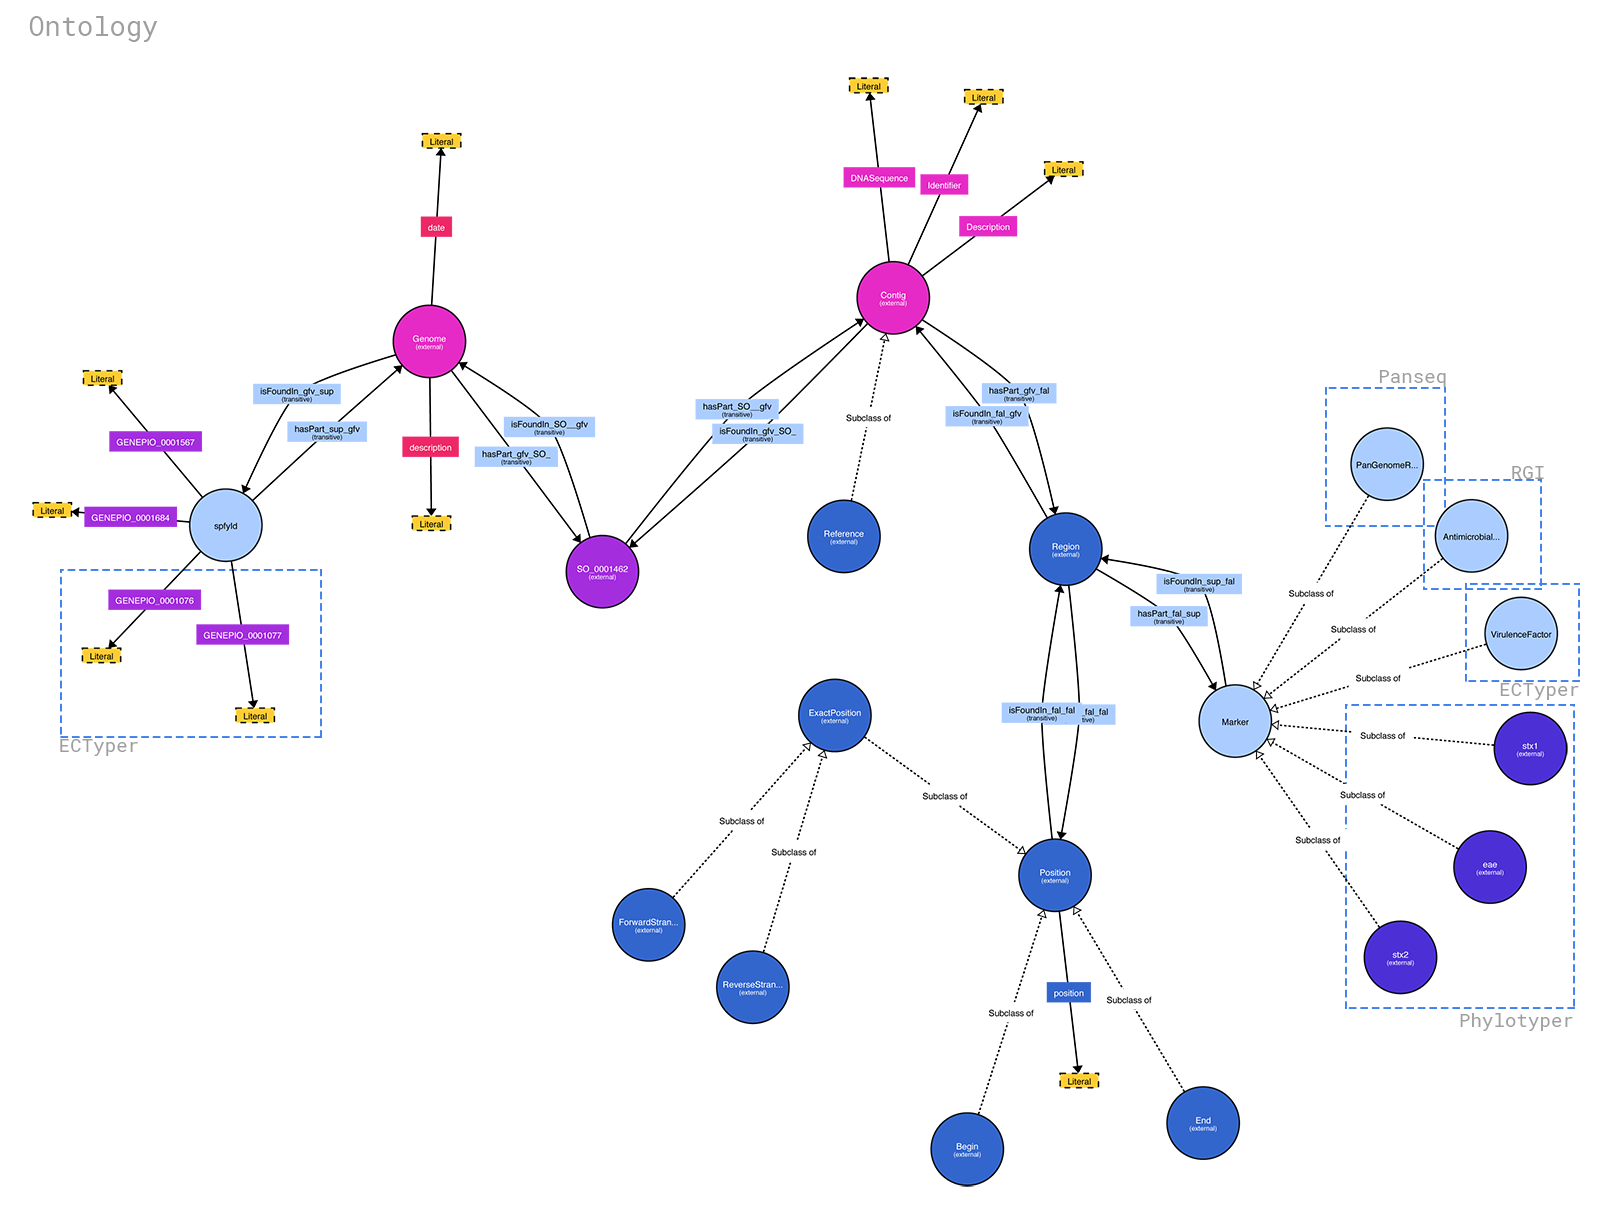
\includegraphics[width=\textwidth]{images/ontology}
\end{center}
\caption{Structure of Spfy's graph database. Brackets highlight the source of different data points and the software it was generated from. These parts are added in as the analyis modules complete, at varying times, and the overall connections are inferred by the database. Non-bracketed sections are sourced from the uploaded genome files or user-supplied metadata.}
\label{fig-ontology}
\end{figure}

% Permanent storage + why a graph is preferable over tables
The permanent storage of results is as a one-time cost to avoid recomputation when the same analysis is re-run. For analyses, Spfy searches the graph for all data points annotated with the queried ontology term. This graph data is then converted into the required structure, usually numerical arrays, or as required for the given analysis module.
In a graph database, a search can begin at any node or attribute. This is in contrast to a SQL database which requires a predefined schema, or a NoSQL database which treats data as documents with varying structure.
For example, the addition of a new analysis module would typically require a new table definition in a SQL database, or the addition of a new document type in a NoSQL database. With a graph database, new nodes or attributes are added and then connected to existing data, removing the need for explicit joins or data conversions. Additionally, data can be added to Spfy in parts, and the database will infer the correct connections between the data.

\subsection{Web design}
% para
% 1. goals: intuitive/familar, ease of use
% 2. design specs
% 3. Google Material design
% 1. implementation: reactjs, react-md, ES6, JSX
% 4. separation from Flask layer

The front-end website is written as a single-page application.
To ensure a familiar user interface, we followed the Material Design specification \url{https://material.io/}, published by Google, surrounding a card-based design.
(see Figure \ref{fig-results})
Both the task selection and result displays follow the same design pattern: while data storage is graph-based, the results of various analysis modules are presented to users in a familiar tabular structure and available for download as .csv spreadsheet files.
(see Figure \ref{fig-tables})

\begin{figure}[!hb]
\begin{center}
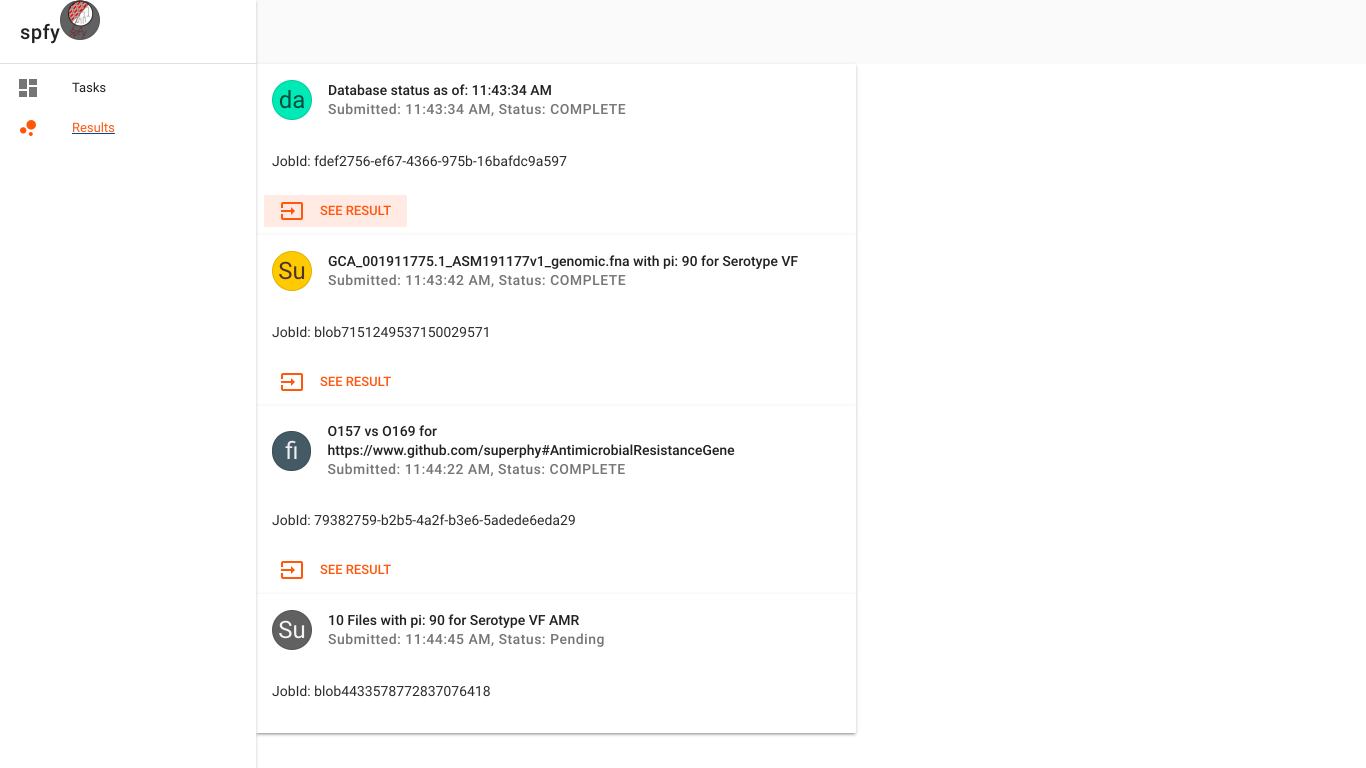
\includegraphics[width=\textwidth]{images/results.png}
\end{center}
\caption{First entry into the results interface for submitted tasks. Cards represent individual tasks and the entire collection can be viewed by sharing the URL with the embedded token.}
\label{fig-results}
\end{figure}

\begin{figure}[!hb]
\begin{center}
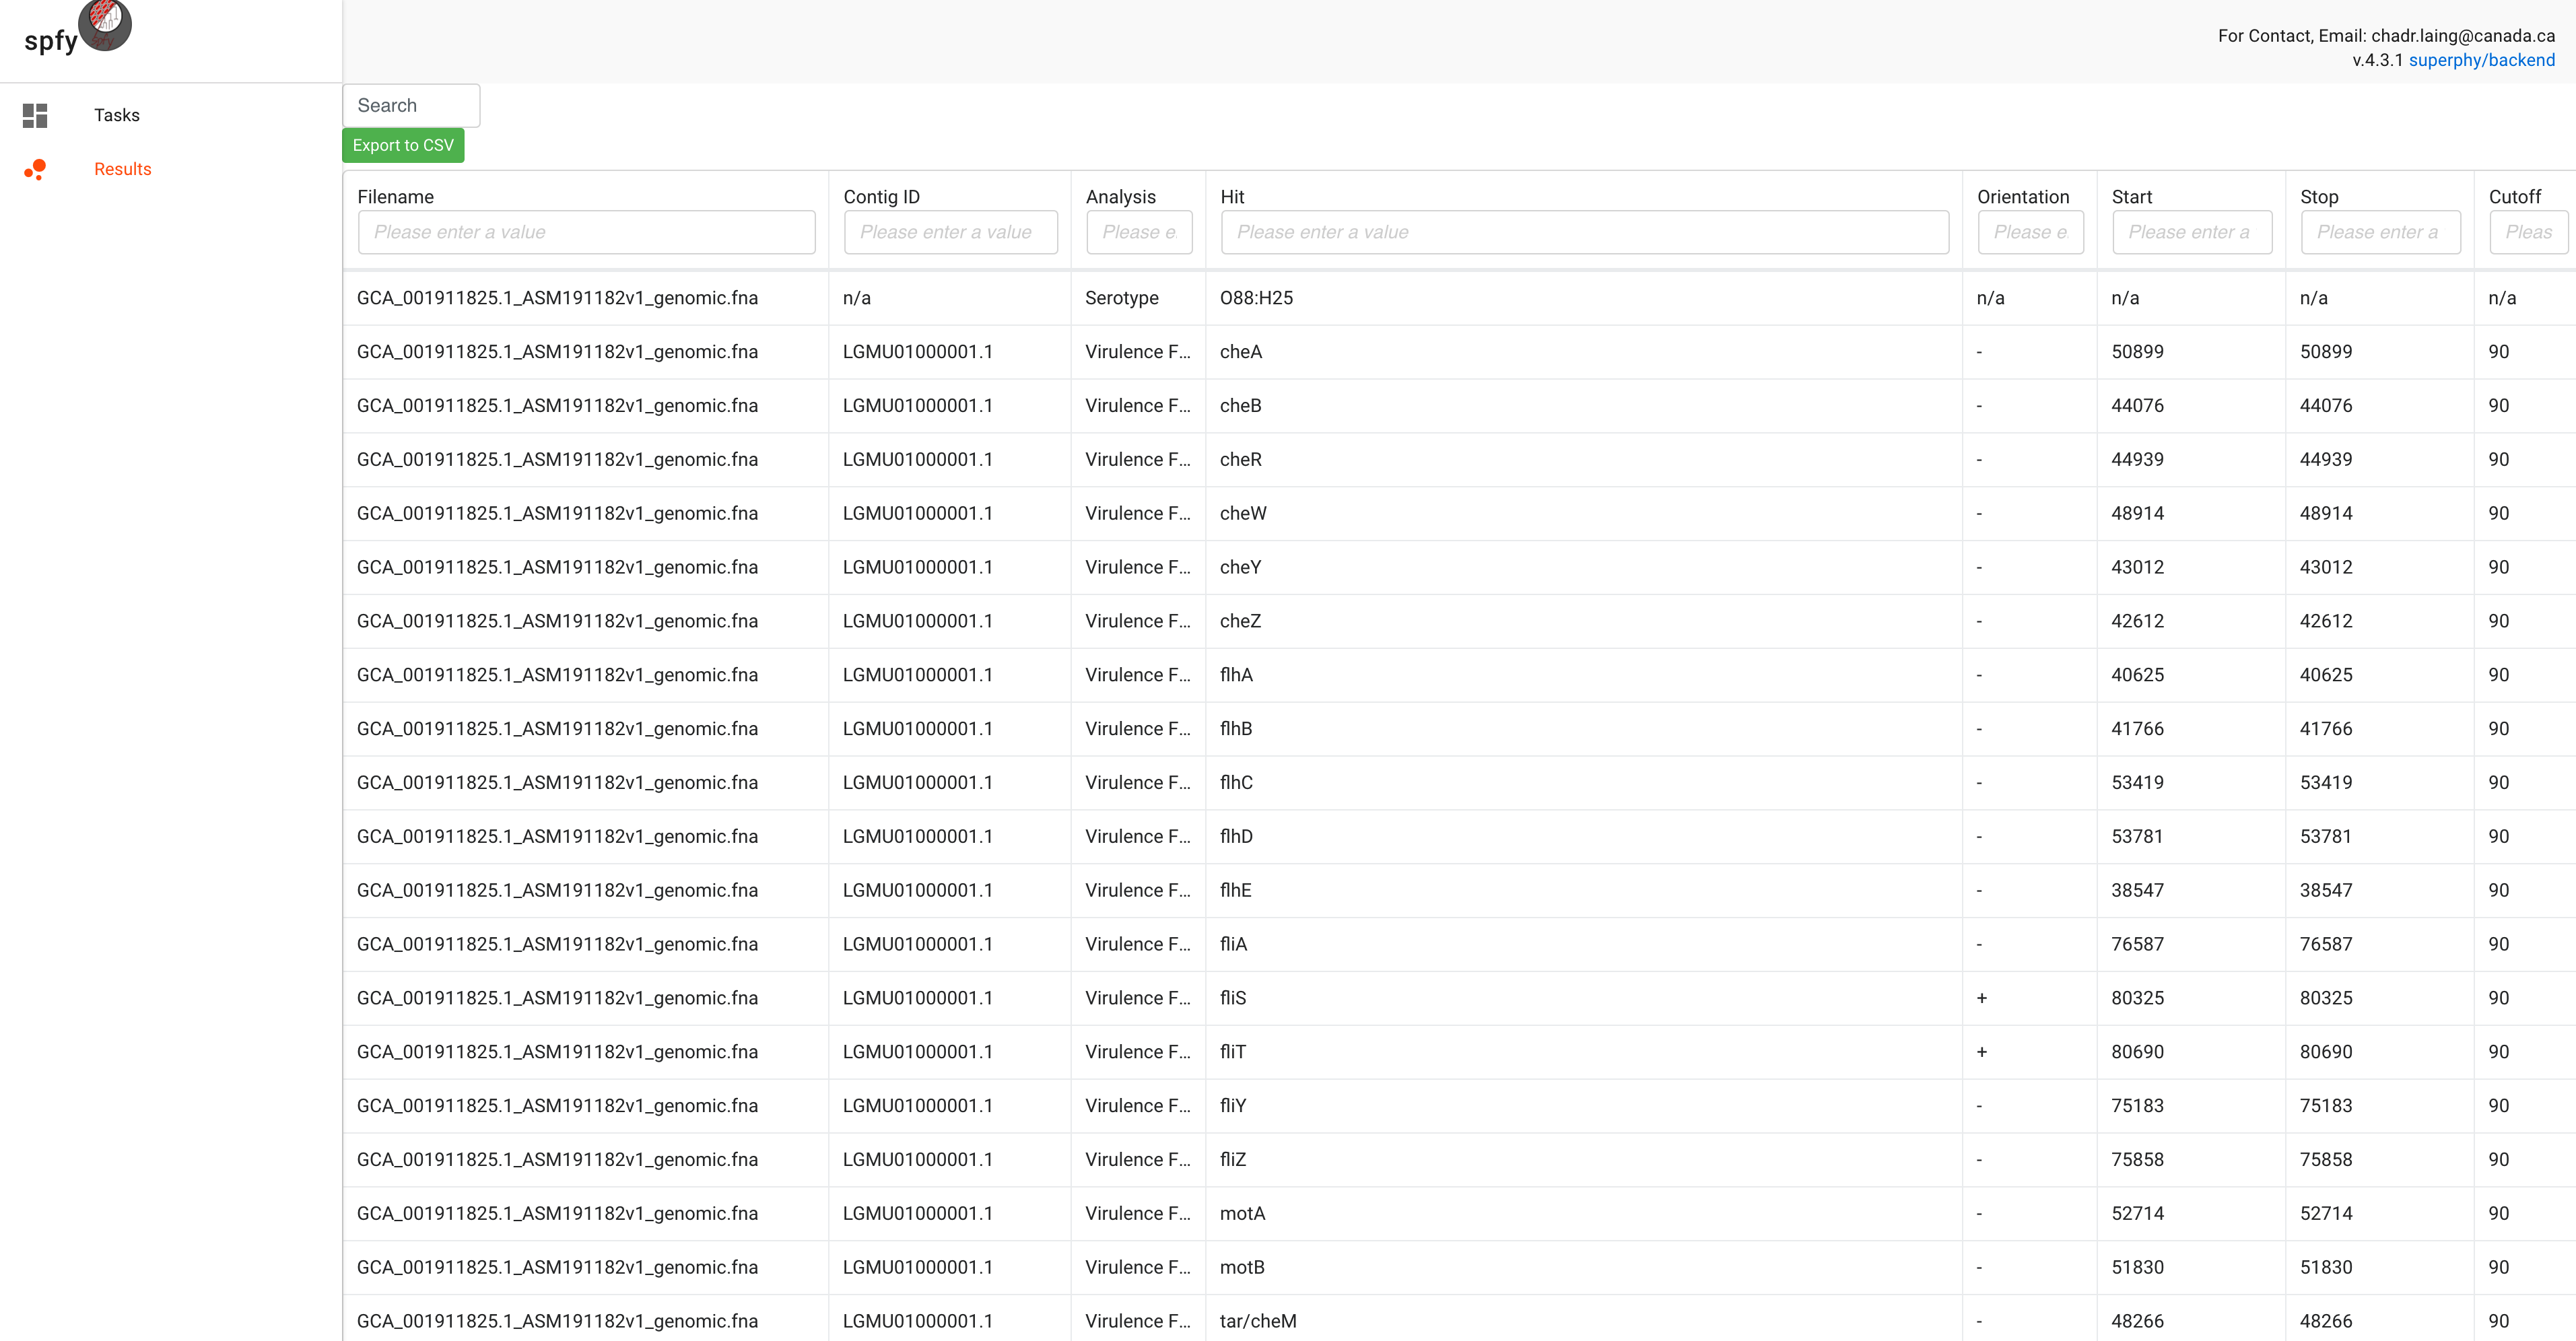
\includegraphics[width=\textwidth]{images/tables.png}
\end{center}
\caption{An expanded result for a subtyping task. While data storage in Spfy is graph-based, a familiar tabular structure is presented to users. The result can also be shared using the URL with the embedded token.}
\label{fig-tables}
\end{figure}

No account creation is required to use the platform. A sharable token is automatically created for users upon entering the website, and is embedded into the website address. Users can share results by copying their URL, and files submitted from different computers using the same token will be visible to anyone with the same link.

\subsection{Service Virtualization}
% para
% 1. goals: real-time, support for pipelines (linked modules)
% 2. how pipelines have been handled in the past: Galaxy, other examples
% 3. Python, RQ
% para
% 1. how we implemented RQ
%	related: packaging of modules in conda

% para
% 1. goals: scale analyses to "big-data", error handling
% 3. how we handle parallelization with RQ
% para
% 1. how many tasks have we tested this with
% 2. error handling: rq-dashboard, sentry
% 3. why options like sentry are better than traditional logging: scales well to tons (big-data levels) of tasks, groups the same errors together, reporting via email

% para
% 1. goals: why compartmentilizations
% 1. how we implemented docker
% 3. how this lets us replicate worker containers and link everything together

% cost of docker < a full VM
% it's not quite a full OS
Docker \url{https://www.docker.com/} is a virtualization technology to simulate self-contained operating systems on the same host computer, without the overhead of full hardware virtualization \cite{felter2015updated}.
The Spfy platform depends on a series of webservers, databases, and task workers, and uses Docker to compartmentalize these services, which are then networked together using Docker-Compose \url{https://docs.docker.com/compose/}.
(see Figure \ref{fig-docker})
Docker integration ensures that software dependencies, which are typically manually installed \cite{doi:10.1093/bioinformatics/btu153,laing2010pan,inouye2014srst2,naccache2014cloud}, are instead handled automatically.

\begin{figure}[!hb]
\begin{center}
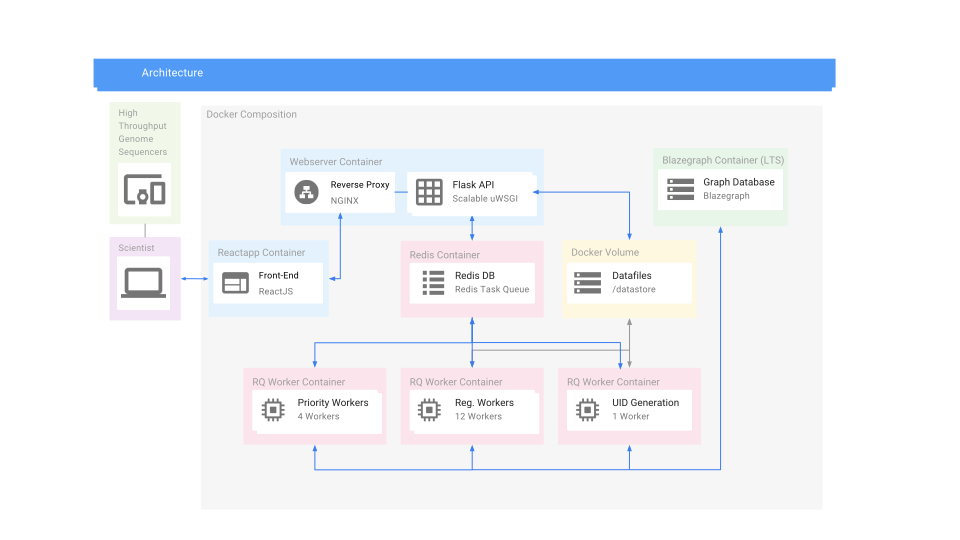
\includegraphics[width=\textwidth]{images/docker}
\end{center}
\caption{The various Docker containers used in Spfy. Arrows represent the connections between different containers, and the entire platform can be recreated with a single command using its Docker-Compose definition.}
\label{fig-docker}
\end{figure}

% standard web tech means you can deploy to different cloud computing services
One of the key benefits of using common-place technologies is the compatibility with other infrastructure resources.
Docker containers are widely supported by cloud computing services: Amazon Web Services (AWS) \url{https://aws.amazon.com/docker/}, Google Cloud Platform (GCloud) \url{https://cloud.google.com/container-engine/}, and Microsoft Azure \url{https://azure.microsoft.com/en-us/services/container-service/}, and self-hosted cloud computing technologies such as OpenStack \url{https://wiki.openstack.org/wiki/Docker}.
% we may want to sign up for a free trial to give an example of this
Spfy packages compute nodes as reproducible Docker containers, and allows the platform to easily scale to demand.

\subsection{Continuous integration}
% Keep this short
% para
% 1. goals: why CI, testing is important
% 2. how we've implemented it, integration with github

Our tests for functionality and backwards compatibility run on TravisCI \url{https://travisci.io}, a continuous integration (CI) platform.
The individual tests use PyTest \url{https://doc.pytest.org/}, and the current build status can be checked either on our GitHub repository or at \url{https://travis-ci.org/superphy/backend}.
TravisCI also builds the core Docker images for Spfy, and uploads them to Docker Hub \url{https://hub.docker.com/u/superphy/}.

\section{RESULTS}
Spfy was tested with 10,243 public \textit{E. coli} assembled genomes from Enterobase, storing every sequence and the results for all included analysis modules. This included: serotypeing (O-antigen, H-antigen), toxin sub-typing (Shiga-toxin 1, Shiga-toxin 2, and Intimin), the identification of VF and AMR determinants, and determination of pan-genome content \textit{E. coli}.
The resulting database had 17,820 nodes and 3,811,473 leaves, with 1,125,909,074 object properties.
Spfy has been up since May 2017. The server accepts assembled \textit{E. coli} genomes with the \textit{.fasta} or \textit{.fna} extensions. Submissions are subjected to quality control, ensuring the submitted genomes are \textit{E. coli} sequences before subsequent analyses are run.
\par

\small \begin{table}[]
\centering
\caption{My caption}
\label{my-label}
\begin{tabular}{llllllllllllllllllllllllllllllllll}
name               & indexType & m    & height & nnodes & nleaves & nentries & nrawRecs & nerrors & nodeBytes & leafBytes & rawRecBytes & totalBytes & avgNodeBytes & avgLeafBytes & avgRawRecBytes & minNodeBytes & maxNodeBytes & minLeafBytes & maxLeafBytes & 64  & 128                   & 192                   & 320                   & 512 & 768                   & 1024 & 2048                 & 3072                  & 4096                & 8192                  & blobs                & newM & curM \\
\_\_globalRowStore & BTree     & 32   & 1      & 1      & 3       & 66       & 0        & 0       & 139       & 6404      & 0           & 6543       & 139          & 2134         & 0139           & 139          & 971          & 3974         & 0.0          & 0.0 & 0.25                  & 0.0                   & 0.0                   & 0.0 & 0.25                  & 0.25 & 0.0                  & 0.25                  & 0.0                 & 0.0                   & 803                  & 32   &      \\
kb.lex.BLOBS       & BTree     & 400  & 1      & 1      & 105     & 27507    & 27507    & 0       & 1419      & 536517    & 391801311   & 392339247  & 1419         & 5109         & 14243          & 1419         & 1419         & 3950         & 7724         & 0.0 & 0.0                   & 0.0                   & 0.0                   & 0.0 & 0.0                   & 0.0  & 0.009433962264150943 & 0.0                   & 0.0660377358490566  & 0.9245283018867925    & 0.0                  & 1180 & 400  \\
kb.lex.ID2TERM     & BTree     & 400  & 2      & 4      & 679     & 135940   & 126070   & 0       & 9186      & 2285517   & 11773580    & 14068283   & 2296         & 3366         & 93             & 84           & 3732         & 3265         & 5071         & 0.0 & 0.0014641288433382138 & 0.0                   & 0.0                   & 0.0 & 0.0                   & 0.0  & 0.0                  & 0.0029282576866764276 & 0.9941434846266471  & 0.0014641288433382138 & 0.0                  & 959  & 400  \\
kb.lex.TERM2ID     & BTree     & 400  & 2      & 3      & 566     & 135940   & 0        & 0       & 19549     & 7568016   & 0           & 7587565    & 6516         & 13371        & 0              & 163          & 10061        & 6319         & 47559        & 0.0 & 0.0                   & 0.0017574692442882249 & 0.0                   & 0.0 & 0.0                   & 0.0  & 0.0                  & 0.0                   & 0.0                 & 0.1265377855887522    & 0.8717047451669596   & 299  & 400  \\
kb.spo.JUST        & BTree     & 1024 & 2      & 12     & 7438    & 4045350  & 0        & 0       & 289345    & 202792383 & 0           & 203081728  & 24112        & 27264        & 0              & 520          & 36563        & 8862         & 71349        & 0.0 & 0.0                   & 0.0                   & 0.0                   & 0.0 & 1.3422818791946307E-4 & 0.0  & 0.0                  & 0.0                   & 0.0                 & 0.0                   & 0.9998657718120806   & 262  & 1024 \\
kb.spo.OSP         & BTree     & 1024 & 2      & 10     & 5637    & 3354502  & 0        & 0       & 100552    & 47560227  & 0           & 47660779   & 10055        & 8437         & 0              & 231          & 15766        & 3871         & 24212        & 0.0 & 0.0                   & 0.0                   & 1.7708517797060386E-4 & 0.0 & 0.0                   & 0.0  & 0.0                  & 0.0                   & 0.21073136178501858 & 0.21692934301398972   & 0.572162210023021    & 731  & 1024 \\
kb.spo.POS         & BTree     & 1024 & 2      & 9      & 5552    & 3354502  & 0        & 0       & 100029    & 27106902  & 0           & 27206931   & 11114        & 4882         & 0              & 218          & 18414        & 2818         & 16447        & 0.0 & 0.0                   & 0.0                   & 1.798237727027513E-4  & 0.0 & 0.0                   & 0.0  & 0.0                  & 0.2138104657435713    & 0.24887610142060781 & 0.481568063297968     & 0.05556554576515015  & 988  & 1024 \\
kb.spo.SPO         & BTree     & 1024 & 2      & 11     & 6056    & 3354502  & 0        & 0       & 123800    & 31663320  & 0           & 31787120   & 11254        & 5228         & 0              & 273          & 20896        & 3423         & 10633        & 0.0 & 0.0                   & 0.0                   & 1.6482610845557937E-4 & 0.0 & 0.0                   & 0.0  & 0.0                  & 0.0                   & 0.21279050601615296 & 0.7667710565353552    & 0.020273611340036263 & 939  & 1024
\end{tabular}
\end{table}




% analysis run-time / throughput with different levels of parallelization
% particularly for statistical tests
% should do a 1 genome = X number VFs, Y number of genomes for Y*X retrieval/analysis

\section{DISCUSSION}
% Gist, we address the the "Limitations" of \cite{de2015trends}.
% Namely:
% 1. Custom formats.
% 2. Use of legacy tech (SQL) means youu can't accomadate "Big-Data" goals.

% drawbacks - big data
Many bioinformatics software programs have been developed \textit{ad hoc}, with individual researchers and laboratories developing software specific to their environment \cite{de2015trends}.
Such tools were often script-based, with custom data formats, and only suitable for small collections of data \cite{de2015trends}.
Recent efforts \cite{goecks2010galaxy,thomsen2016bacterial} have focused on providing a common web interface for these programs, while still returning the same result files.
However, many subsets of biology now require the analyses of big-data, where inputs are taken from a variety of analysis programs, and involve large-scale data warehousing \cite{schatz2015biological}.
The ability to integrate data from different source technologies, merge submissions from other labs, and distribute computations over fault-tolerant systems are now required for types of analyses that need to be performed \cite{schatz2015biological}.

One of the key goals in developing Spfy was to accommodate and store a variety of result formats, and then to make the data from these results retrievable and usable as inputs for downstream analyses, such as predictive biomarker discovery. We have shown how a graph database can accommodate the results given by a variety of bioinformatics programs, and how Spfy is performant for data retrieval on the results for multiple analyses among over 10,000 genomes, providing results from big-data comparisons in the same efficiency as old analyses on single files.

\mwcomment{I think this discussion sets the perfect tone for the big data applications provided by spfy. My only suggestion is to give examples of the types analysis that are mentioned in the review. One idea, instead of dropping "Impact on Public Heath Efforts" entirely, you can convert it into a use case example that highlights the benefit spfy provides.}

\subsection{Impact on Public Heath Efforts}

% para
% focus on application
The isolation and characterization of bacterial pathogens are critical for Public Health laboratories to rapidly respond to outbreaks, and to effectively monitor known and emerging pathogens through surveillance programs.
Until recently, public-health agencies relied on laboratory tests such as serotyping, pulsed-field gel electrophoresis (PFGE), PCR-based amplification of known VFs, and disc-diffusion assays to identify AMR, for the characterization of bacterial isolates in outbreak, surveillance, and reference laboratory settings \cite{ronholm2016navigating}. Current efforts are focused on predictive genomics, where the relevant phenotypic information can be determined through examination of the whole-genome sequence without need for the traditional laboratory test.

Spfy provides rapid and easy predictive genomic analyses of \textit{E. coli} genomes while also addressing the problem of large scale comparisons. With the larger datasets involved in population genomics, it is no longer viable for individual researchers to download data to perform comparisons. Instead, efforts have focused on storing biological data online and enabling analyses on that data \cite{schatz2015biological}. By using a graph database, Spfy can integrate results from  different technologies including software predicted phenotypes as well as laboratory results and user-submitted metadata. In addition, datasets can be built and submitted from multiple labs for joint analysis. 

\subsection{Comparison with other bioinformatic pipeline technologies}
% trying to cut down on details that would be better suited for the "Implemntation" section.


% namely galaxy
The automated analyses of WGS is currently facilitated by existing scientific workflow technologies such as Galaxy \cite{goecks2010galaxy}. Galaxy aims to provide a reproducible, computational interface which is accessible to individuals without programming knowledge. Galaxy defines a formal schema for linking different analysis software together, so the entire analysis pipeline can be replicated and also extended as new analysis tools are developed. The Galaxy worklow focus is on running an individual analysis pipeline. It does not include functionality to store and collate analysis results for large-scale comparative analysis.

The Bacterium Analysis Pipeline (BAP) \cite{thomsen2016bacterial} provides an integrated analysis pipeline for bacterial WGS data as a web service. It provides an individual per-genome report of the determined species, multilocus sequence type, VF and AMR genes \cite{thomsen2016bacterial}.

Spfy is similar to these technologies in that it automates workflows for users, and as in Galaxy, uses task queues to distribute selected analyses.
% re: Matt "2. When comparing to IRIDA, BAP etc., can mention some differences with Superphy, e.g. the storage of interim result data that allows downstream integrated analysis"
On a per file basis, Spfy performs at a similar speed to BAP on predictive genomics tasks, though Spfy does not provide genome assembly services.
Spfy processes XXXX files over XX tasks in XXXX time, distributing computations over a task queue and multiple Docker compartmentalized containers.
However, unlike these workflow managers, Spfy is designed to help solve the needless recomputation of analyses by storing results in a graph database for downstream comparative analysis. This allows Spfy to perform population-wide analyses, regardless of the individual analysis software used to generate the results for an individual genome.

\small % Please add the following required packages to your document preamble:
% \usepackage{graphicx}
\begin{table}[!hb]
\centering
\caption{Comparison of various bioinformatic pipelines and their underlying database. Functionally, Spfy integrates different analysis modules as in BAP while also merging large datasets as in PATRIC.}
\label{Table 2.}
\resizebox{\textwidth}{!}{%
\begin{tabular}{lllll}
         & Spfy                & Galaxy              & BAP                 & PATRIC              \\
Database & Blazegraph          & PostgreSQL          & MySQL + File System & MongoDB + Shock     \\
Type     & Graph               & SQL                 & SQL + File System   & NoSQL               \\
Focus    & Integrated Analyses & Workflow Technology & Batch Analysis      & Integrated Analyses
\end{tabular}%
}
\end{table}


PATRIC \cite{wattam2016improvements} adds support for comparing up to nine user-submitted genomes against a reference genome, targeting various gene annotations. PATRIC indexes a NoSQL document store to compare similar document types and is beneficial for comparative genomics. Unlike PARTIC, Spfy is targeted towards statistical comparisons of any population grouping, and Spfy's graph database has no limit on the number of genomes grouped for comparison. For example, Spfy can compare all genomes with a particular subtype for gene annotations, source metadata targets for gene annotations, or any two (or more) node or attribute types as shown in \ref{fig-groupings}.

\begin{figure}[!hb]
\begin{center}
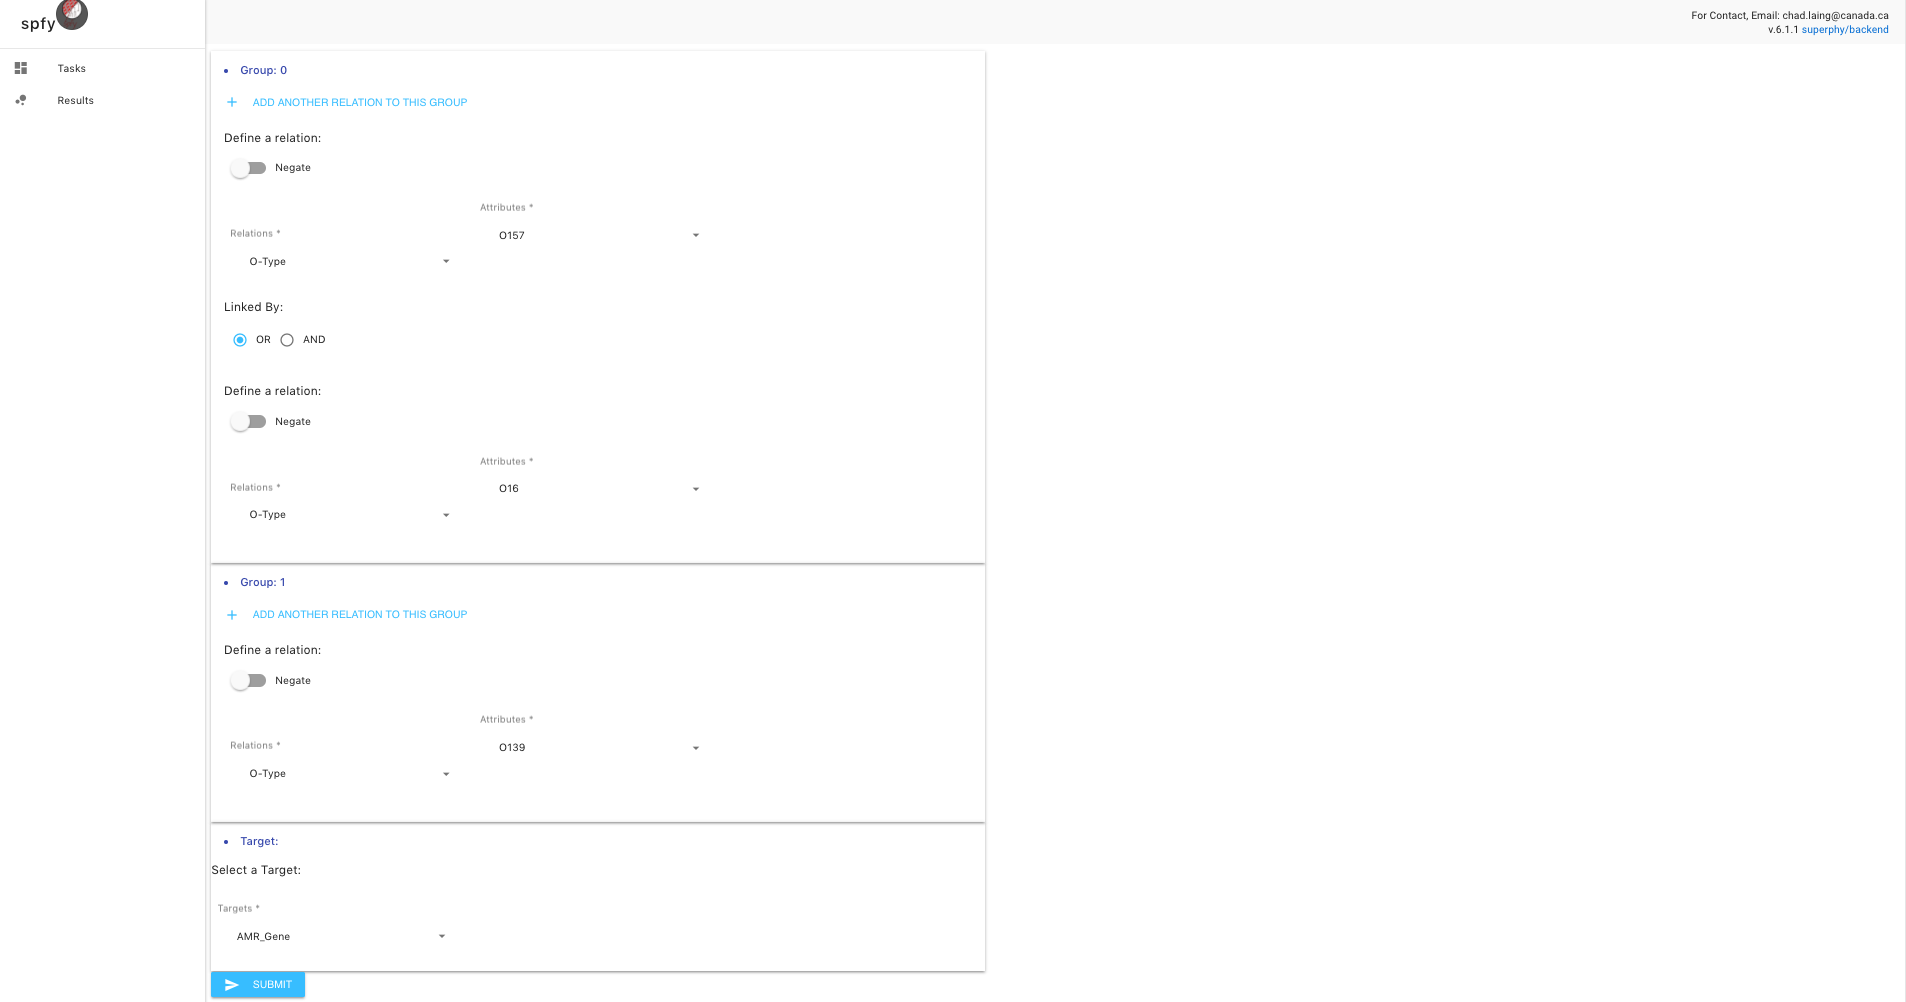
\includegraphics[width=\textwidth]{images/groupings}
\end{center}
\caption{Genomes can be grouped by any node or attribute type for comparisons, and Spfy has no upper bound for the number of genomes in a group. Different types can also be joined into a group through logical connectives AND, OR, Negation, and any data type is also a valid target. This approach can be used to compare any data regardless of source software.}
\label{fig-groupings}
\end{figure}

\mwcomment{Maybe should include a comparison to PATRIC. Patric does offer some comparative genomic analysis, however they are not health focused (pathways, gene presence/absence etc), and you cannnot add your own data to the repository}

\section{CONCLUSIONS}

Future work will focus on adding additional analyses modules to aid genotype to phenotype predictions using machine learning modules, and supporting bacterial species such as \textit{Salmonella}, and \textit{Campylobater}. While the integrated approach of storing and retrieving results provides enormous benefits, the developed analyses modules are self-contained and be transfered to existing platforms such as Galaxy. The source code for Spfy is hosted at \url{https://github.com/superphy/backend}, and is available for free under the open-source Apache 2.0 license. A developer guide is provided at \url{https://superphy.readthedocs.io/en/latest/}.

\textit{Conflict of interest}. None declared.

\section{ACKNOWLEDGEMENTS}

\newpage

\bibliographystyle{unsrt}
\bibliography{paper-webserver}

\newpage

\section{APPENDIX}

\end{document}
